\documentclass{article}
\usepackage[a4paper,margin=1in]{geometry}
\usepackage{amsmath, amsfonts, amssymb, amstext, mathtools, stmaryrd, textcomp, xcolor, graphicx, tikz}
\usepackage[hidelinks]{hyperref}
\usetikzlibrary{automata, positioning, arrows, trees}
\tikzset{->,>=stealth,
every state/.style={thick, fill=gray!10}, 
initial text=$ $,
}
\newcommand{\e}{\varepsilon}
\newcommand{\s}{\Sigma}
\newcommand{\g}{\Gamma}
\newcommand{\so}{\rightarrow}
\newcommand{\str}{\texttt}
\newcommand{\newp}{\\[2mm]}
\newcommand{\defeq}{\coloneqq}
\newcommand{\spc}{\textvisiblespace}

\title{Homework 05}
\author{Aaron Wang}
\date{March 21 2025}

\begin{document}
\maketitle
\begin{enumerate}
    \item \textbf{Non-closure properties of CFLs}
    \begin{enumerate}
        \item [(a)][Exercise 2.2a] Use the languages
        \[
            A=\{\str{a}^m\str{b}^n\str{c}^n|m,n \geq 0\}
        \]
        \[
            B=\{\str{a}^n\str{b}^n\str{c}^m|m,n \geq 0\}
        \]
        to prove that context-free languages are not closed under intersection. \newp
        \begin{figure}[ht]
\centering
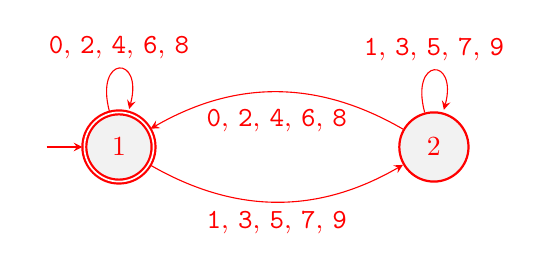
\begin{tikzpicture}
\color{red}
    \node[state, initial, accepting] (q1) {1};
    \node[state, right of=q1, xshift=3cm] (q2) {2};
    \draw (q1) edge[loop above] node[]{\str{0}, \str{2}, \str{4}, \str{6}, \str{8}} (q1)
    (q2) edge[loop above] node[]{\str{1}, \str{3}, \str{5}, \str{7}, \str{9}} (q2)
    (q2) edge[bend right] node[below, yshift=-0.1cm]{\str{0}, \str{2}, \str{4}, \str{6}, \str{8}} (q1)
    (q1) edge[bend right] node[below]{\str{1}, \str{3}, \str{5}, \str{7}, \str{9}} (q2);
\end{tikzpicture}
\end{figure}
        \item [(b)][Exercise 2.2b] Use Problem 1a and DeMorgan’s law to prove that context-free languages are \textit{not} closed under complementation. \newp
        \begin{figure}[ht]
\centering
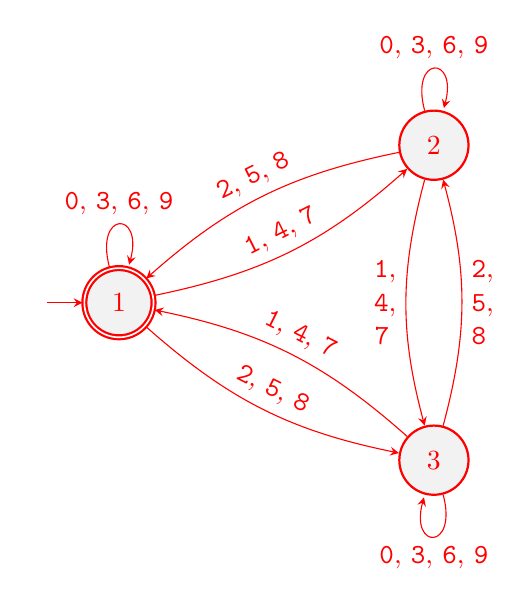
\begin{tikzpicture}
\color{red}
    \node[state, initial, accepting] (q1) {1};
    \node[state, right of=q1, xshift=3cm, yshift=2cm] (q2) {2};
    \node[state, right of=q1, xshift=3cm, yshift=-2cm]  (q3) {3};
% go forward one node  
    \draw (q1) edge[bend right=15] node[sloped, above]{\str{1}, \str{4}, \str{7}} (q2)
    (q2) edge[bend right=15] node[left, align=center]{\str{1},\\ \str{4},\\ \str{7}\:} (q3)
    (q3) edge[bend right=15] node[sloped, above]{\str{1}, \str{4}, \str{7}} (q1)
% go back one node     
    (q1) edge[bend right=15] node[sloped, above]{\str{2}, \str{5}, \str{8}} (q3)
    (q3) edge[bend right=15] node[right, align=center]{\str{2},\\ \str{5},\\ \str{8}\;} (q2)
    (q2) edge[bend right=15] node[sloped, above]{\str{2}, \str{5}, \str{8}} (q1)
% looping nodes
    (q1) edge[loop above] node[above]{\str{0}, \str{3}, \str{6}, \str{9}} (q1)
    (q2) edge[loop above] node[above]{\str{0}, \str{3}, \str{6}, \str{9}} (q2)
    (q3) edge[loop below] node[below]{\str{0}, \str{3}, \str{6}, \str{9}} (q3)
    ;     
\end{tikzpicture}
\end{figure}
    \end{enumerate}
\newpage
    \item \textbf{There and back again.} Imagine a robot turtle that you can give instructions \str{u} (go up 1 cm), \str{d} (go down 1 cm), \str{l} (go left 1 cm), \str{r} (go right 1 cm). A program is a string of instructions.\newp
    Let $C$ be the set of programs that make the turtle return to its starting point. For example, \str{uurdrdll} is in $C$, as shown in this picture:
    \begin{center}
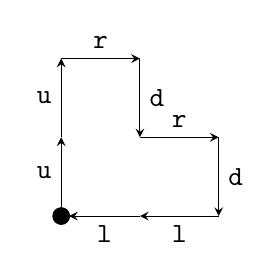
\begin{tikzpicture}
    \filldraw[black] (0,0) circle (3pt);
    \draw[->] (0,0.1) -- (0,1) node[midway,left] {\str{u}}; 
    \draw[->] (0,1) -- (0,2) node[midway,left] {\str{u}};
    \draw[->] (0,2) -- (1,2) node[midway,above] {\str{r}};
    \draw[->] (1,2) -- (1,1) node[midway,right] {\str{d}}; 
    \draw[->] (1,1) -- (2,1) node[midway,above] {\str{r}};
    \draw[->] (2,1) -- (2,0) node[midway,right] {\str{d}}; 
    \draw[->] (2,0) -- (1,0) node[midway,below] {\str{l}}; 
    \draw[->] (1,0) -- (0.1,0) node[midway,below] {\str{l}}; 
\end{tikzpicture}
\end{center}
    \vspace{-10mm}
    \begin{enumerate}
        \item Prove that $C$ is not context-free.\newp
        \begin{figure}[h]
\centering
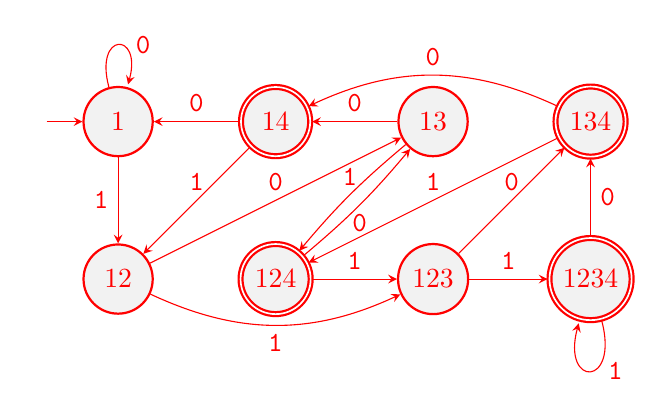
\begin{tikzpicture}
\color{red}
    % \node[state, initial] (q000) {$q_{000}$};
    % \node[state, yshift=-2cm] (q001) {$q_{001}$};
    % \node[state, xshift=4cm] (q010) {$q_{010}$};
    % \node[state, yshift=-2cm, xshift=4cm] (q011) {$q_{011}$};
    % \node[state, xshift=2cm, accepting] (q100) {$q_{100}$};
    % \node[state, yshift=-2cm, xshift=2cm, accepting] (q101) {$q_{101}$};
    % \node[state, xshift=6cm, accepting] (q110) {$q_{110}$};
    % \node[state, yshift=-2cm, xshift=6cm, accepting] (q111) {$q_{111}$};
    \node[state, initial] (q000) {1};
    \node[state, yshift=-2cm] (q001) {12};
    \node[state, xshift=4cm] (q010) {13};
    \node[state, yshift=-2cm, xshift=4cm] (q011) {123};
    \node[state, xshift=2cm, accepting] (q100) {14};
    \node[state, yshift=-2cm, xshift=2cm, accepting] (q101) {124};
    \node[state, xshift=6cm, accepting] (q110) {134};
    \node[state, yshift=-2cm, xshift=6cm, accepting] (q111) {1234};
    \draw 
        (q000) edge[loop above] node[right, xshift=1mm]{\str{0}} (q000)
        (q000) edge[] node[left]{\str{1}} (q001)
        (q001) edge[] node[above]{\str{0}} (q010)
        (q001) edge[bend right=25] node[below]{\str{1}} (q011)
        (q100) edge[] node[above]{\str{0}} (q000)
        (q100) edge[] node[above]{\str{1}} (q001)
        (q101) edge[bend right=5] node[below]{\str{0}} (q010)
        (q101) edge[] node[above]{\str{1}} (q011)
        (q010) edge[] node[above]{\str{0}} (q100)
        (q010) edge[bend right=5] node[above]{\str{1}} (q101)
        (q011) edge[] node[above]{\str{0}} (q110)
        (q011) edge[] node[above]{\str{1}} (q111)
        (q110) edge[bend right=25] node[above]{\str{0}} (q100)
        (q110) edge[] node[above]{\str{1}} (q101)
        (q111) edge[] node[right]{\str{0}} (q110)
        (q111) edge[loop below] node[right, xshift=1mm]{\str{1}} (q111)
    ;
\end{tikzpicture}
\end{figure}
        \item Write a \textbf{formal description} of a Turing machine that decides $C$.\newp
        \answer{
    Run $TM_{L2}$ on $\langle TM_{L2} \rangle$. Assume towards a contradiction that $TM_{L2}$ is 10-compliant. Thus we will be at step 4 and simulate $TM_{L2}$ on $\langle TM_{L2} \rangle$. This should either accept or reject.
    \begin{itemize}
        \item [] If $TM_{L2}$ accepts $\langle TM_{L2} \rangle$, then we must reject $\lightning$. 
        \item [] If $TM_{L2}$ rejects $\langle TM_{L2} \rangle$, then we must accept $\lightning$.
    \end{itemize}
    Since we have a contradiction, $TM_{L2}$ must not be 10-compliant.
}
    \end{enumerate}
\newpage
    \item \textbf{Turing closure properties.} Let $\s = \{\str{0}, \str{1}\}$. Recall in HW2 we defined
        \[
        \text{STRETCH}(w_1w_2 \cdots w_n) = w_1w_1w_2w_2 \cdots w_{n-1}w_{n-1}w_nw_n. 
        \]
        for any string $w_1w_2 \cdots w_n \in \s^*$ This induces an operation on languages,
        \[
        \text{STRETCH}(L) = \{\text{STRETCH}(w) | w \in L\}.  
        \]

    \begin{enumerate}
        \item Write an \textbf{implementation-level} description of a Turing machine $S$ that, on input $v \in \s^*$, decides whether $v = \text{STRETCH}(u)$ for some $u$. Moreover, if $S$ accepts $v$, then when it halts, the contents of the tape should be $u$. For example, if the input is \str{001100}, $S$ should accept and the final contents of the tape should be \str{010}. But if the input is \str{001101}, $S$ should reject.\newp
        \textcolor{red}{
The following is an NFA for B. The Intuition is this. First let's consider $k=1$. In this case, all we need is a $w$ that contains one \str{1}. Now consider, what if we thought $k$ was 2 or $s=\str{1}^2w$. Let us rewrite it as $s=\str{1}w'$ s.t. $w'=\str{1}w$. Now we have the same case as before. For any $k > 1$, we could do this such that $s=\str{1}^kw=\str{1}^1w'$ s.t. $w' = \str{1}^{k-1}w$. In essence, we now realize that we are looking only for a string that starts with \str{1} and contains at least 2 \str{1}s.
}
\begin{figure}[h]
\centering
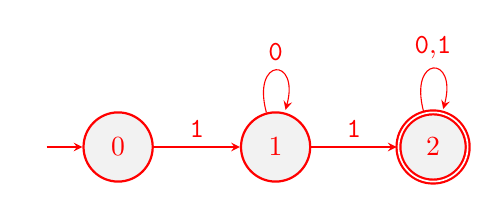
\begin{tikzpicture}
\color{red}
    \node[state, initial] (q0) {0};
    \node[state, xshift=2cm] (q1) {1};
    \node[state, xshift=4cm, accepting] (q2) {2};

    \draw
    (q0) edge[] node[above]{\str{1}} (q1)
    (q1) edge[loop above] node[above]{\str{0}} (q1)
    (q1) edge[] node[above]{\str{1}} (q2)
    (q2) edge[loop above] node[above]{\str{0},\str{1}} (q2)
    ;
\end{tikzpicture}
\end{figure}
        \item Prove that if $L$ is a Turing-decidable language over $\s$, then STRETCH$(L)$ is also Turing-decidable. You should let $M$ be a Turing machine that decides $L$, then use your answer to 3a to give an \textbf{implementation-level} description of a Turing machine that decides STRETCH$(L)$. One of the lines of your description can be ``Simulate $M$.''\newp
        \textcolor{red}{
Let $M'$ be the Turing machine that describes STRETCH$(L)$\newp
$M' = $ ``On input string $w$''
\begin{quote}
\begin{enumerate}
    \item[1.] Simulate S
    \item[2.] If $S$ rejects $w$: \emph{reject}.
    \item[3.] If $S$ accepts $w$: Move head to start of tape\footnote{In the case that this is too high level, what one could do is add a preprocessing step, Mark the first two symbols, Run S, and then at this point rewind to marked symbol, unmark it and continue.} and simulate M on the current tape.
    \item[4.] \emph{accept} or \emph{reject} as $M$ would.
\end{enumerate}
\end{quote}
}
        \item Prove that if $L$ is a Turing-recognizable language, then STRETCH$(L)$ is also Turing-recognizable.\newp
        \textcolor{red}{
Use the same answer as (b) with one change: 4. \emph{accept}, \emph{loop}, or \emph{reject} as $M$ would.\newp
This change is necessary because $M$ can now loop so $M'$ can as well.
}
    \end{enumerate}
\end{enumerate}
\end{document}